\section{Frontend}
\label{desenvolupament:frontend}
Al llarg de les següents línies es descriurà, de la mateixa manera que s'ha fet a la secció \ref{dev_backend}, l'evolució del projecte al llarg de la durada del Treball de Final de Grau; concretament, aquesta secció contemplarà les decisions preses durant el desenvolupament i l'avanç del projecte, en la seva component \textit{front-end}.\\
\newline Tot i que aquesta part del projecte no ha patit canvis tan importants com els explicats anteriorment, si que s'ha hagut d'adaptar el funcionament a les noves necessitats que han aparegut a mesura que s'ha avançat.\\

\subsection{Model incial}
En un primer moment, recordem que la plataforma depenia d'una entitat anomenada tercer de confiança que s'ocupava principalment de la certificació i firma dels consentiments informats generats per la plataforma \textit{Made of Genes}.
Per aquesta raó, en primera instància, es buscava que la part client fos una mera visualització del document generat i que permetés a l'usuari acceptar del document generat.\\
%\newline Recordem que el consentiment informat és un contracte en el qual s'expliciten totes els detalls relatius al tractament/estudi que es realitzarà, possibles efectes, alternatives i demés; per tant, és de vital importància que el client el visualitzi.\\
\newline A la següent figura (fig.\ref{fig:front_init}) es pot veure un primer \textit{mockup} del que s'esperava que fos el client:
\begin{figure}[h]
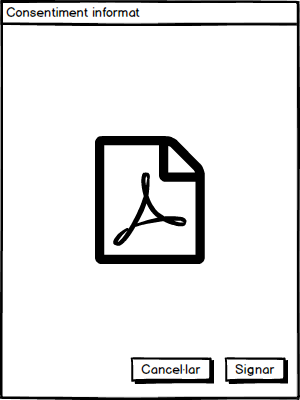
\includegraphics[scale=0.4]{sections/developement/init_front.png}
\centering
\caption{Mockup inicial del \textit{front-end}}
\label{fig:front_init}
\end{figure}
\newline Com es pot veure a la figura anterior, el client disposa d'un visualitzador de documents .pdf i un parell de botons:
\begin{itemize}
    \item Cancel·lar, tal i com indica el seu nom servirà per cancel·lar el procés de signatura. L'usuari el podrà reprendre en qualsevol altre moment.
    \item Signar, aquest botó porta a acceptar el consentiment i a iniciar el procés de signatura del document.
\end{itemize}
La simplicitat de la interfície es deu a que el gruix del procés el porta a terme el tercer de confiança a través del correu electrònic.\\

\subsection{Model final}
De la mateixa manera que a la secció anterior del capítol, no poder integrar finalment els serveis del tercer de confiança suposa un canvi dràstic en les mecàniques de funcionament, el \textit{frontend} ha patit lleugeres modificacions per a poder satisfer els nous requisits.\\
\newline A la Figura \ref{fig:cas_us_frontend}, es mostren els casos d'ús del \textit{frontend}, són quatre:
\begin{itemize}
    \item Visualitzar consentiment informat.
    \item Validar identitat del signant.
    \item Signar consentiment informat.
    \item Demanar nou OTP.
\end{itemize}
La figura següent mostra un nou \textit{mockup} sobre el \textit{frontend} del projecte, que satisfà els quatre casos d'ús anteriors:
\begin{figure}[h]
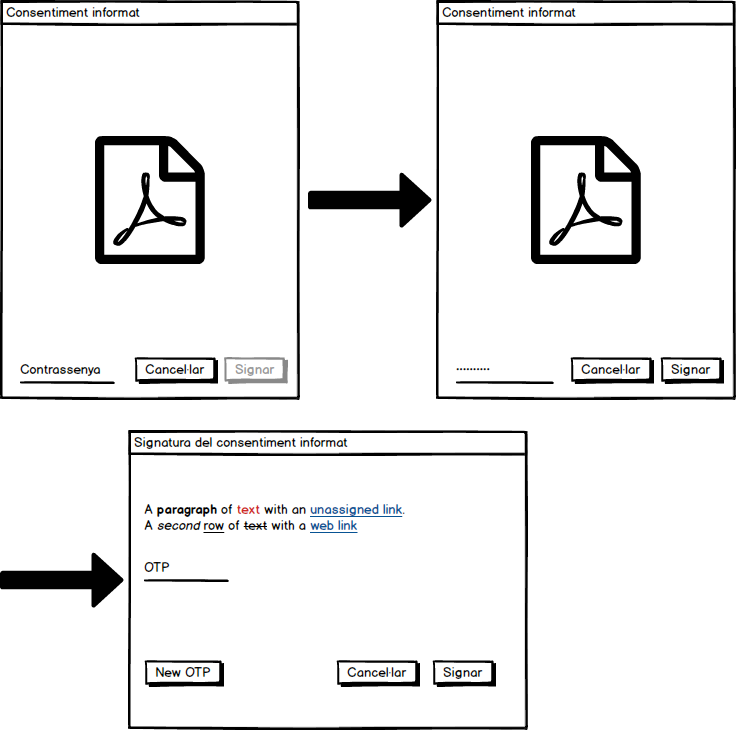
\includegraphics[scale=0.4]{sections/developement/final_front.png}
\centering
\caption{Mockup final del \textit{frontend}}
\label{fig:front_final}
\end{figure}
\newline Altre cop, cal dir que la simplicitat del disseny ve donada per la complexitat dels processos que s'executen al \textit{backend} i dels que l'usuari, no n'ha de ser partícep a excepció d'aquells que requereixin estrictament una interacció per part seva, com poden ser inserir el codi OTP o validar la seva identitat.\\
\clearpage
Les següents captures formen part del procés de signatura d'un consentiment informat en un entorn de producció:
\begin{figure}[h]

\includegraphics[scale=0.5]{sections/developement/sms_otp.jpg}
\centering
\caption{SMS amb el codi OTP per signar}
\label{fig:sms:otp}
\end{figure}
\begin{figure}[h]
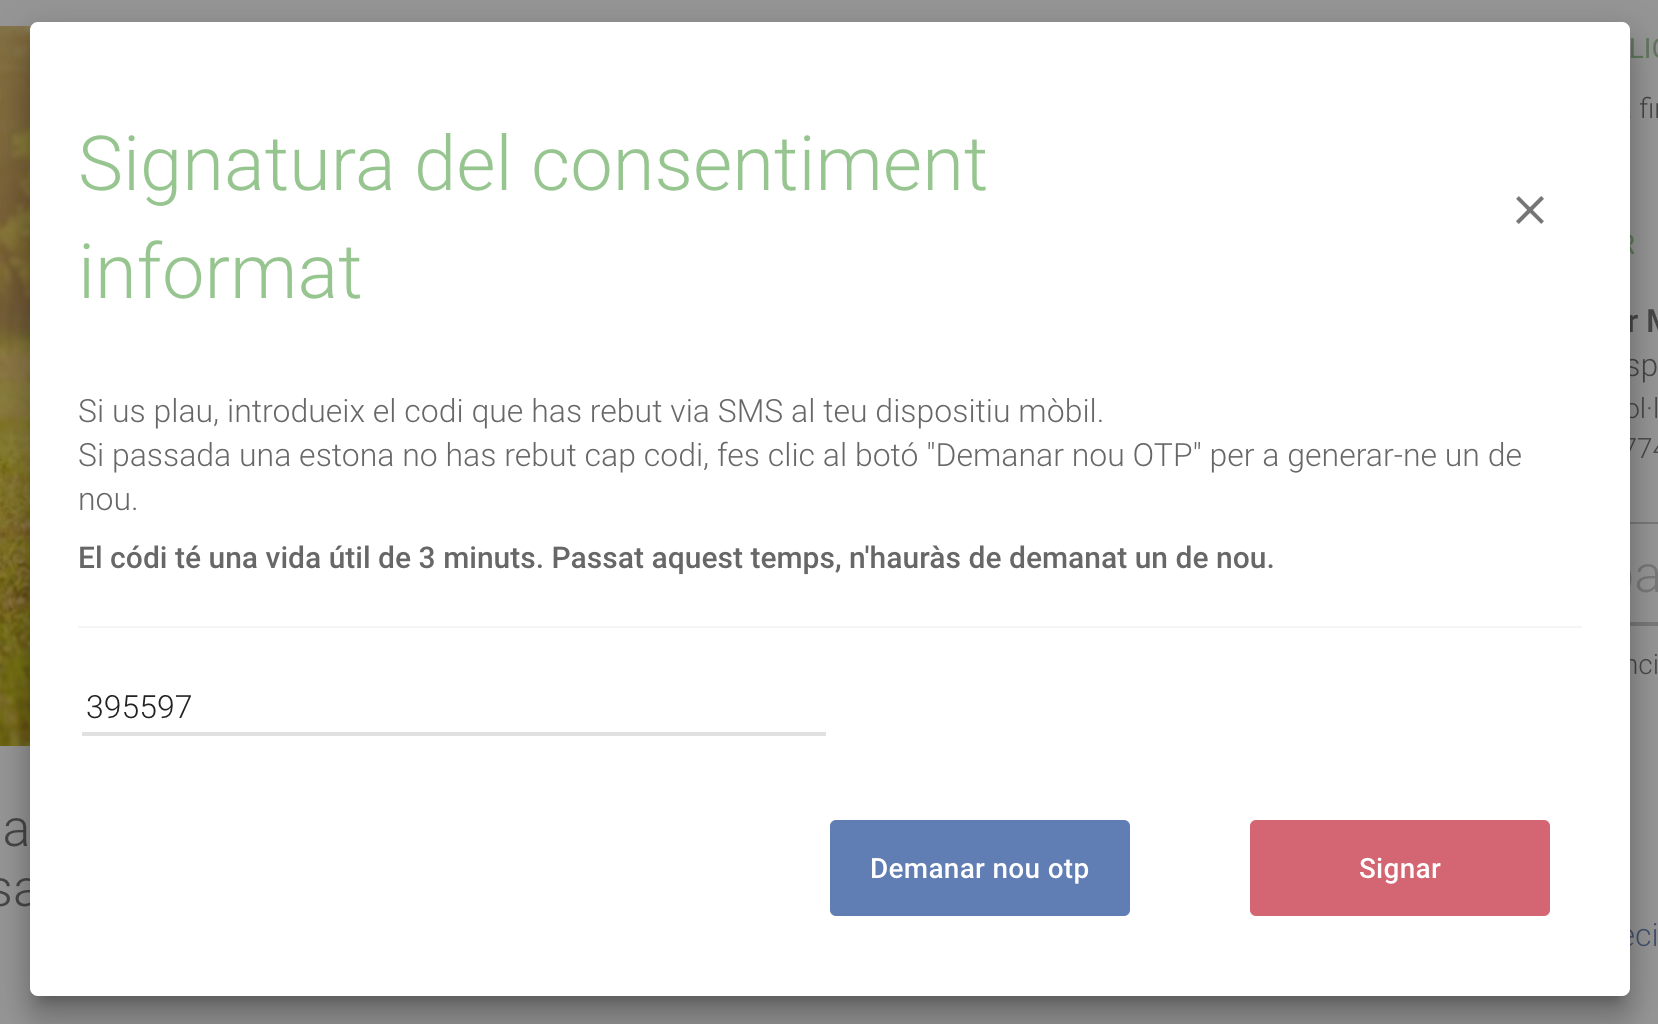
\includegraphics[scale=0.5]{sections/developement/frontend_otp.png}
\centering
\caption{Popup de signatura del consentiment informat}
\label{fig:front_init}
\end{figure}



%Aquests canvis, com no pot ser d'una altre forma, tenen conseqüències al \textit{frontend}.\\
%Tot i no poder-se comparar amb els canvis 


%\newline Aquest procés, és totalment transparent a l'usuari, tret del moment en el que rep per part del tercer de confiança el correu electrònic corresponent al consentiment informat certificat i el codi OTP amb el qual signarà l'esmentat document.\\
%\clearpage
%El funcionament del tercer de confiança és el següent:
%\begin{enumerate}
%    \item L'usauri prem al botó de "Signar"
%    \item L'usuari rep un correu electrònic on hi trobarà dos coses: 
%    \begin{itemize}
%        \item Consentiment informat segellat per l'entitat
%        \item Link a la pàgina web de signatura
%    \end{itemize}
%    \item En cas d'estar d'acord amb el contingut del consentiment presentat, prem sobre el vincle del correu i entrarà a una pàgina web per a signar el document
%    \item El tercer de confiança envia un codi OTP a l'usuari.
%    \item L'usuari introduirà el codi rebut via SMS al camp corresponent dins del lloc web
%    \item \textbf{El document queda signat i certificat}
%\end{enumerate}
%Tenint en compte l'anterior correlació d'esdeveniments es pote entendre el disseny simple, ja que els que requereix és permetre a l'usuari llançar el procés de signatura del document.\\
%\newline No obstant les facilitats que ens ofereix el tercer de confiança, apareixen problemes que








%\subsection{Primers passos}
%Com bé s'ha descrit en capítols anteriors, la part del client de la plataforma es desenvolupa amb \textit{AngularJS}.\\
%Inicialment, l'experiècnia de l'autor amb tecnologies d'ambit web era més aviat inexistent, així que mentre es recollien les dades necessàries per a començar amb els esbossos i el disseny del document de requisits finals, es va aprofitar per indagar i recopilar informació sobre el llenguatge (Javasctipt), sobre el qual no es disposava de l'experiència suficient per a dur a terme amb soltura un projecte d'aquest caire així com agafar una mica de pràctica amb lús i beneficis del \textit{framework} que es fa servir a l'empresa.

%\subsection{Inici del desenvolupament}
%Un cop redactat el document de requisits, especificats els diferents casos d'ús i tenir una primera versió dels diferents dissenys, comença el que es pot considerar una primera fase de desenvolupament.
%\newline En aquesta fase, es porta a terme un projecte des de zero.
%\newline El desemnvolupament d'aquest projecte suposa el gruix principal del dsencolupament del frontend, ocupant gran part del temps dedicat.
%\subsection{Fase final}
%Finalment, es porta aterme la esmentada integració del mòdul que forma part del TFG a la plataforma \textit{Made of Genes}.
%\newline Aquest procés d'integració suposa tot un seguit de canvis dins del projecte inicial.
%\newline Tot i els canvis, no hi han hagut deviacions que hagin afectat seriament al procés del projecte, i s'ha pogut finalitzar a temps



% explicar que es planteja com una finestra emergent que permet a l'usuari signar el consentiment informat que se li mostra mitjançant la seva contrassenya  de la plataforma i un codi OTP 